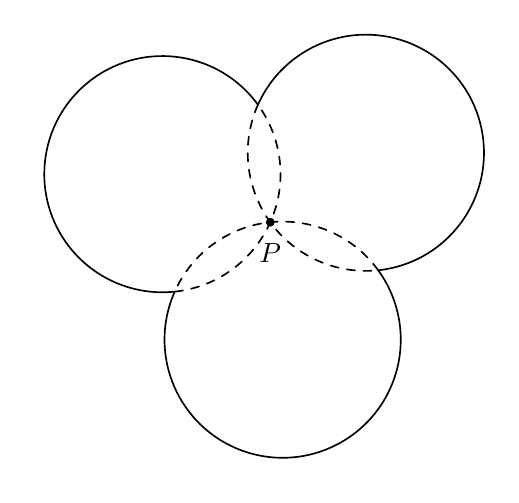
\begin{tikzpicture}[x=1cm,y=1cm,line width=0.6pt,line join=round,line cap=round,rotate=6]

\coordinate (O1) at ({-1.5*sqrt(3)/2},.75);
\coordinate (O2) at ({1.5*sqrt(3)/2},.75);
\coordinate (O3) at (0,-1.5);
\coordinate (P) at (0,0);
\draw (O1) ++(30:1.5) arc (30:270:1.5);
\draw (O2) ++(270:1.5) arc (270:510:1.5);
\draw (O3) ++(150:1.5) arc (150:390:1.5);
\draw[dashed] (O1) ++(270:1.5) arc (270:390:1.5);
\draw[dashed] (O2) ++(150:1.5) arc (150:270:1.5);
\draw[dashed] (O3) ++(30:1.5) arc (30:150:1.5);
\fill (P) circle (1.6pt);
\node[below=2pt,xshift=0.00bp,yshift=-2.00bp] at (P) {$P$};
\end{tikzpicture}
